\section{Preliminary Evaluations} \label{sec:results}

This chapter presents and discusses the preliminary results accomplished by the proposed method so far. First, \methodname results in the training stage are presented, including the loss and metrics computed. Secondly, we discuss the performance of the proposed method in the FICV competition. Then, the \methodname is compared against the best results achieved by the methods shown in Chapter \ref{sec:literature}. Finally, we analyze some visualizations performed over the proposed method to understand its predictions.

\subsection{Training Performance}

In this subsection, we discuss the training performance regarding the \icao requirements followed by the results of eye landmarks detection. We focus on analysing  the loss charts and values of metrics described in Chapter \ref{sec:measures}.

\subsubsection{Requirements}

We start by presenting the results of \methodname during the training phase. The \autoref{fig:losses} shows the loss in training and validation sets for unsupervised and supervised branches individually. As can be seen, the loss of unsupervised branch was lower and smoother than the supervised during the whole training. This behaviour was expected since (i) the reconstruction task performed by the unsupervised branch is theoretically more straightforward than the multi-label classification carried out by the supervised branch, and (ii) the unsupervised loss has a higher weight during training (see section \ref{sec:hyperparams} and \autoref{eq:loss-final}). 

A more detailed analysis of our loss curves shows that \methodname presented an appropriate balance between bias and variance. In the unsupervised branch, both train and validation loss are approximately zero and similar to each other. Therefore, the network achieved a notable performance in reconstructing the input image from the shared embeddings. Similarly, even though the losses from the supervised branch are more significant than the unsupervised one, they are still close to zero. However, we can notice a noisier loss curve regarding the validation set. Although such loss curves present a higher variance, they keep near the training curve through the epochs. Furthermore, the overfitting was prevented by the regularization techniques employed during training, i.e., batch normalization, dropout layers, Early Stopping, and the architecture itself (as detailed in Section \ref{sec:hyperparams}).

\begin{figure}[ht]
\centering
\subfigure[unsupervised]{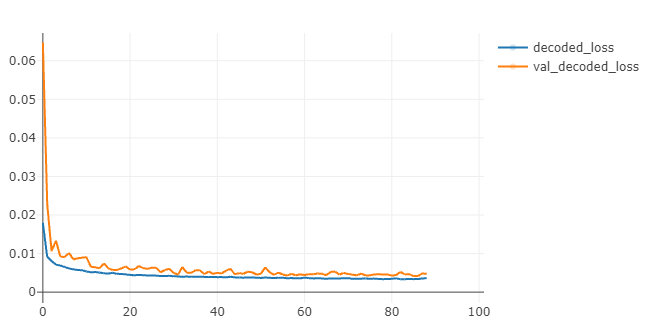
\includegraphics[width=0.8\linewidth]{images/graphs/loss_unsupervised.png}}
\hfill
\ContinuedFloat
\subfigure[supervised]{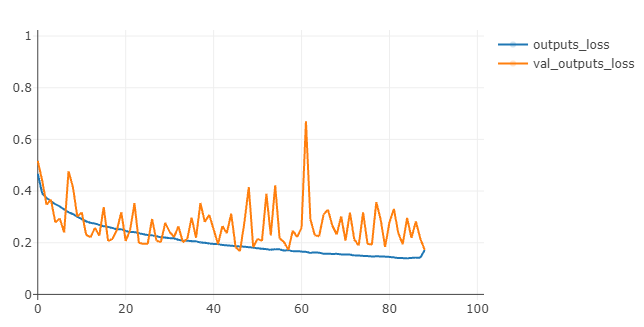
\includegraphics[width=0.8\linewidth]{images/graphs/loss_supervised.png}}
\caption{Loss of training and validation sets for (a) unsupervised and (b) supervised branches. Source: own elaboration.}
\label{fig:losses}
\end{figure}

The final metrics of \methodname are given in \autoref{tab:metrics}, where some meaningful insights about the proposed method can be observed. First, it is better to predict the compliant requirements (positive class) than the non-compliant since the Precision and Recall are higher than the \acs{npv} and Specificity. Probably, this is influenced by the unbalanced dataset. Moreover, the \acl{fp} predictions (type-I error) are a more critical problem of \methodname because both Recall and \acs{npv} are greater than Precision and Specificity, respectively. In particular, the Specificity indicates that a reasonable amount of non-compliant requirements are being assigned as compliant. On the other hand, the proposed method achieved considerably high values of F-measure and F-beta, which shows a fair balance between Precision and Recall. Finally, the notable \acs{mcc} score (82.78) indicates that the \methodname was able to learn valuable patterns for both compliant/non-compliant requirements even with the unbalancing present in the \adhoc database.

\begin{table}[H]
\centering
\caption{Global metrics of \methodname achieved in the best training epoch.}
\label{tab:metrics}
\begin{tabular}{@{}cc@{}}
\toprule
\textbf{Metric} & \textbf{Value (\%)} \\ \midrule
Accuracy & 94.27 \\
Precision & 94.53 \\
Recall & 97.89 \\
F-measure & 96.15 \\
F-beta & 97.14 \\
NPV & 91.67 \\
Specificity & 81.69 \\
MCC & 82.78 \\ \bottomrule
\end{tabular}
\end{table}

\subsubsection{Eye Location Accuracy} \label{sec:eye_location_acc}

In contrast to the intuition, the detection of eye landmarks revealed to be a harder task than the assessment of \icao requirements. The \autoref{fig:eye-training} presents the Wing loss and eye location accuracy ($d_{eye} \in [0;0.1[$) in training and validation sets. In contrast to the supervised branch for requirements, we can notice the presence of bias in the loss graph during training (the loss is far away from zero), indicating the network was not able to learn useful patterns and detect eye landmarks accurately. Such behaviour also happens in the validation set. Nonetheless, these results also reflect in the eye location accuracy metric, which reach the maximum value of $46.18\%$ in the \adhoc dataset. 

\begin{figure}[ht]
\centering
\subfigure[Wing Loss]{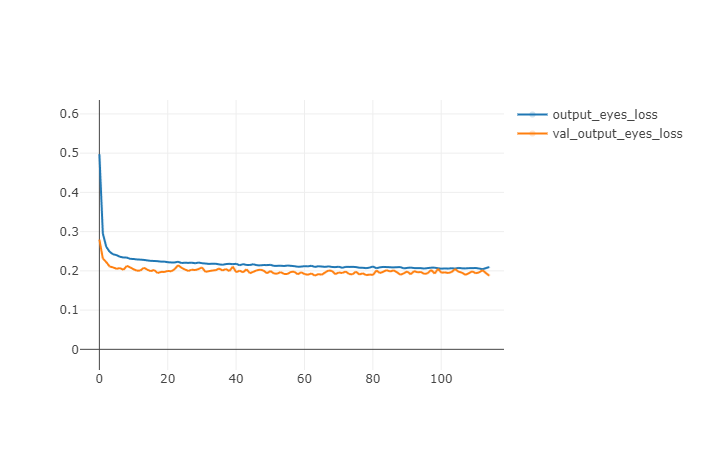
\includegraphics[width=0.8\linewidth]{images/graphs/loss_eyes.png}}
\subfigure[Eye Localization Accuracy]{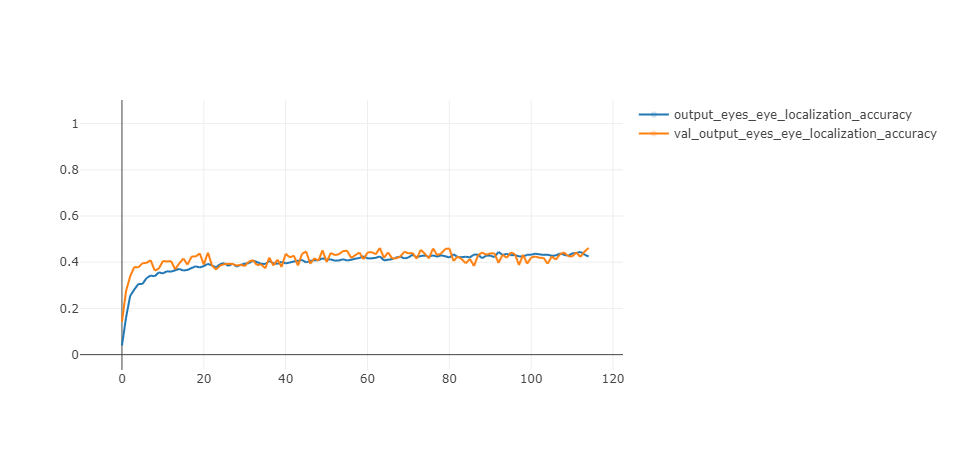
\includegraphics[width=0.8\linewidth]{images/graphs/eyes_location_accuracy.png}}
\caption{Results of eye localization for training and validation sets: (a) wing loss and (b) $d_{eye} \in [0;0.1[$. Source: own elaboration.}
\label{fig:eye-training}
\end{figure}

A sample of images with the landmarks predicted by \methodname is shown in \autoref{fig:eyes_detection}. In the first two rows, there are arbitrary examples of most precise detections (i.e., $d_{eye} \in [0;0.1[$). We can observe that \methodname can perform accurate detections for frontal face images even with the presence of requirements that could potentially harm accurate localization of the landmarks. For example, we can see the presence of images with \framecoveringeyes and \toodarklight. On the other hand, in the last two rows, there are samples of the worst detections, i.e. $d_{eye} \geq 0.3$. In this case, an evident pattern of highly rotated face images (\rollpitchyaw) is perceptible. Furthermore, the presence of other requirements can be noticed (e.g, \blurred and \framestooheavy).

\begin{figure}[h]
\centering
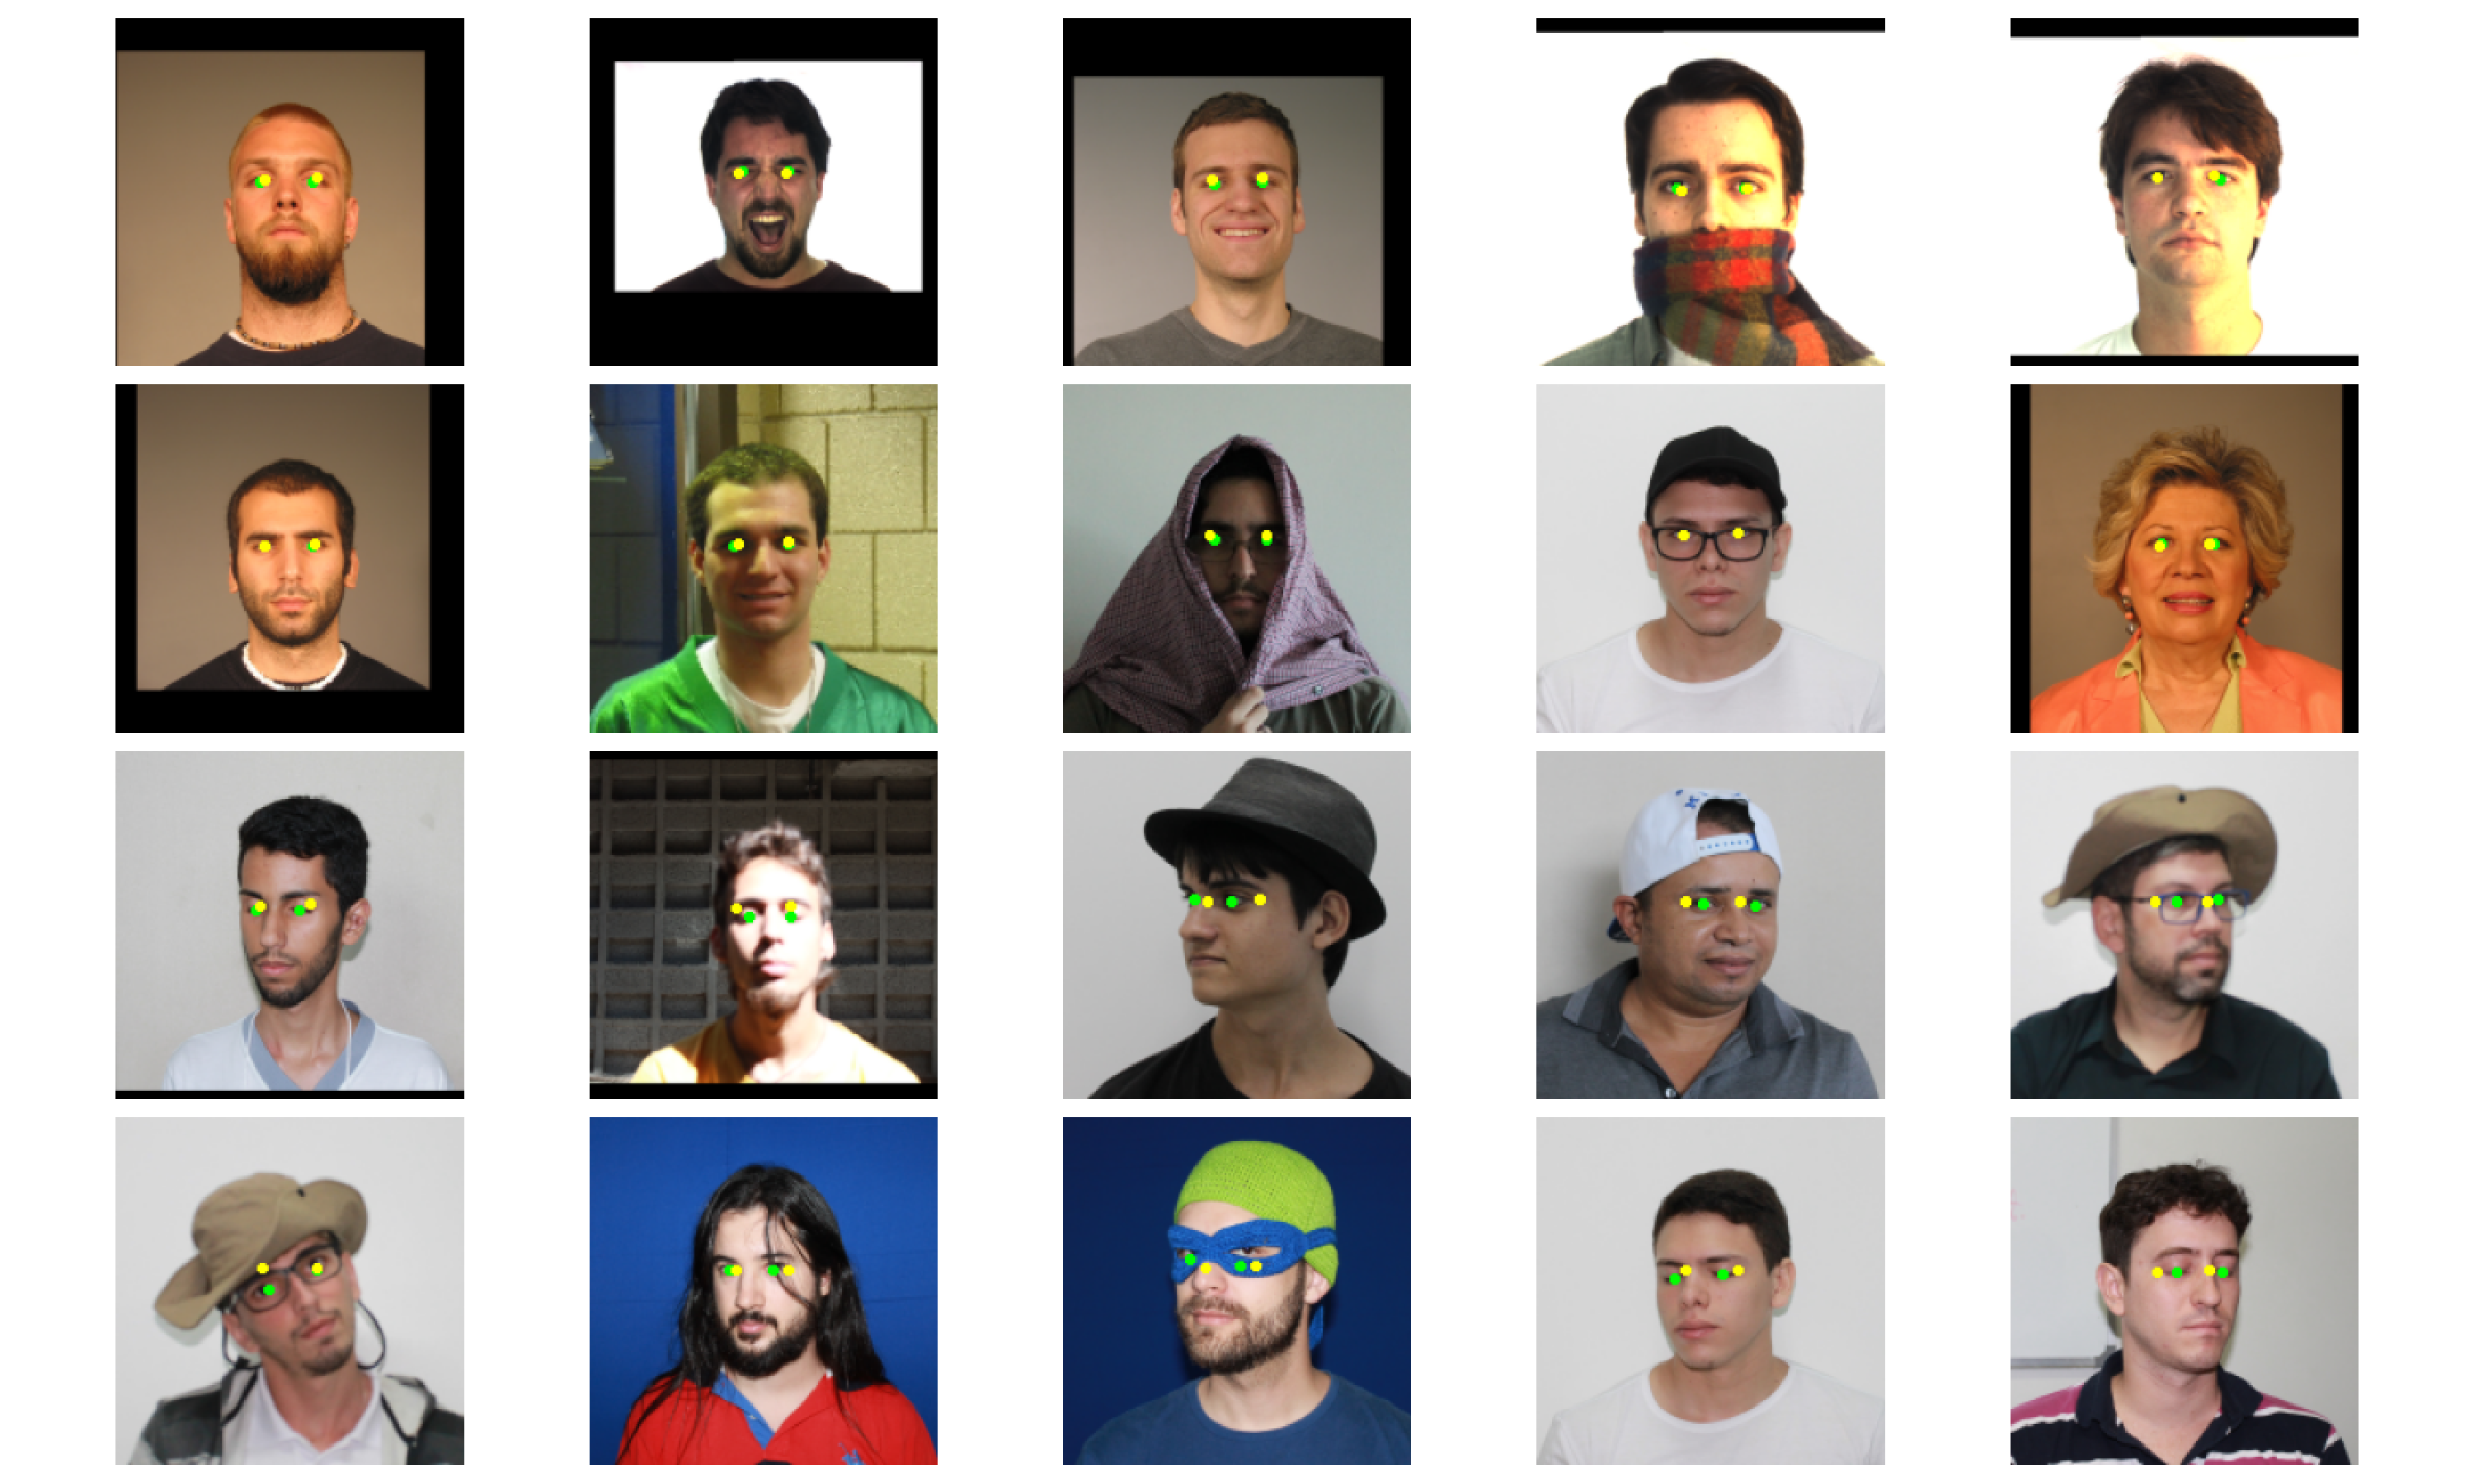
\includegraphics[width=\linewidth]{images/eyes/detections.pdf}
\caption{Results of eyes landmarks detection by \methodname. The first two rows contains images with $d_{eye} \in [0;0.1[$, and the last rows are for $d_{eye} \geq 0.3$. The ground-truth annotations are shown in green, while network predictions are in yellow.}
\label{fig:eyes_detection}
\end{figure}

We analysed the network predictions for eye landmarks to understand the bias observed during training. In \autoref{fig:heatmap_eyes}, we can see a heatmap of landmarks in the validation set. As can be noticed, there are two noticeable clusters for each eye, indicating that the networks is essentially predicting landmarks over the same regions regardless the input image. We suppose this behaviour is caused mainly by the preprocessing step, which centers the face in the input image.

Moreover, we presume the low performance in eye landmark localization can be explained by one or more reasons from below:

\begin{figure}[h]
\centering
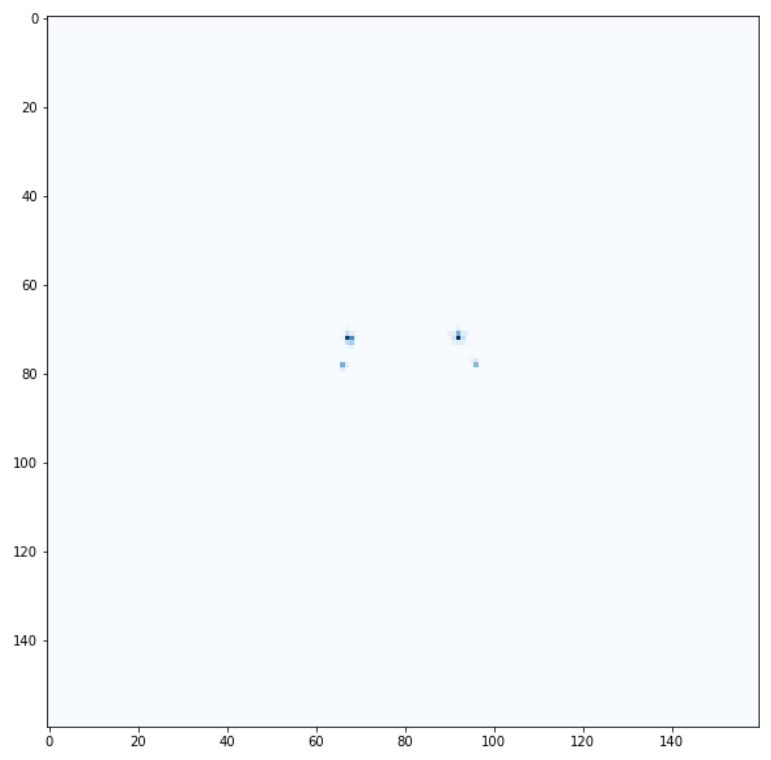
\includegraphics[width=0.6\linewidth]{images/eyes/heatmap_eyes_v0.914.png}
\caption{Heatmap of detected eye landmarks in the \adhoc dataset.}
\label{fig:heatmap_eyes}
\end{figure}

\begin{enumerate}[i]
\item \textbf{Preprocessing}: our preprocessing method centralize the face by creating a region around it (see Section \ref{sec:preprocessing}). Therefore, the network can be inducted to predict the mean of landmark positions to minimize the loss function. However, we tried to apply different levels of image augmentation in other experiments. Although the predictions were more distributed over the image, there was no significant changes in the loss and location accuracy.

\item \textbf{Dataset}: our \adhoc image dataset is mostly composed by images with frontal faces with little variation in face poses and alignment. In addition, the amount of images (approximately five thousand) is noticeably low in comparison with other landmarks datasets. For example, there are more than 200 thousand images with labeled landmarks in the 300-VW \citep{tzimiropoulos2015project} or CelebFaces \citep{yang2015facial} datasets. In fact, we ran some experiments with a subset of CelebFaces dataset as our training set (and left the entire \adhoc dataset as validation). In all of them, overfitting was achieved (i.e., high performance in training, but low performance in validation). We believe it comes from the fact that the patterns found in CelebFaces dataset are even easier than in ours. All faces are centered and with corrected orientation (the last is not carried out by our preprocessing step). Again, as mentioned before, we tried data augmentation, but it did not help to improve overall performance.

\item \textbf{Embeddings}: when training the branch for detection of eye landmarks, the remaining parts of \methodname architecture was frozen, including the encoder and corresponding embeddings. We could argue that (i) the embeddings does not contain helpful representation of the eyes that can be relevant for landmark detection; and (ii) it can be harmful to the landmarks branch since it would not have the chance to update the embeddings. Despite of it, we already had empirical evidence that the embeddings contains useful information of the eyes before training the landmarks branch. Later is this work, we will see the regions closer to eyes are important for requirements assessment (see Section \ref{sec:netviz}).

\item \textbf{Training Components}: we ran tests with \acs{mse}, Wing Loss, and $d_{eye}$ as both loss functions and metrics for early stopping.  After all, \methodname was not able to predict the landmarks accurately. It goes against to other works found in the literature that also applies multitask learning for facial landmarks prediction (e.g., \citep{zhang2014facial, ranjan2017hyperface, zhang2015learning}. On the other hand, we could have leveraged the use of more advanced losses and models. It will be left for future works though.

\end{enumerate}

In conclusion, considering the scope of the possible reasons mentioned above, we suspect the dataset is the main problem for the low performance on eye localization accuracy. Therefore, by improving the data with more variations in face pose, location and orientations, the results may be improved. Nevertheless, further investigation must be conducted to verify this hypothesis.


\subsection{Results in the FICV Competition} \label{sec:ficv_results}

In \autoref{tab:icaonet-ficv}, we can see the \acl{eer} and Rejection Rate for each FICV dataset. In the \ficvtest, the method proposed was able to achieve a perfect \acs{eer} in eight requirements (08, 11, 12, 16, 23, 24, 28, and 29). In the \ficvofficial dataset, it happened only in the \veiloverface, even though most of the other results are considerably low. 

\begin{table}[tb]
\centering
\caption{Results of \methodname according to the benchmark of the FICV competition. The EER and Rejection Rate are shown in percentage.}
\label{tab:icaonet-ficv}
\begin{tabular}{@{}clrrrr@{}}
\toprule
\multirow{2}{*}{\textbf{Req. \#}} & \multicolumn{1}{c}{\multirow{2}{*}{\textbf{Requirement description}}} & \multicolumn{2}{c}{\textbf{FICV-TEST}} & \multicolumn{2}{c}{\textbf{FICV-1.0}} \\ \cmidrule(l){3-6} 
 & \multicolumn{1}{c}{} & \multicolumn{1}{c}{EER} & \multicolumn{1}{c}{Rej.} & \multicolumn{1}{c}{EER} & \multicolumn{1}{c}{Rej.} \\ \midrule
\textbf{08} & Blurred & 0.00 & 0.00 & 2.10 & 0.60 \\
\textbf{09} & Looking away & 5.00 & 0.00 & 5.40 & 0.00 \\
\textbf{10} & Ink marked/creased & 46.70 & 0.00 & 49.00 & 0.00 \\
\textbf{11} & Unnatural skin tone & 0.00 & 0.00 & 1.70 & 0.00 \\
\textbf{12} & Too dark/light & 0.00 & 0.00 & 1.20 & 0.00 \\
\textbf{13} & Washed out & 1.50 & 0.00 & 7.30 & 0.00 \\
\textbf{14} & Pixelation & 26.70 & 0.00 & 29.00 & 0.00 \\
\textbf{15} & Hair across eyes & 4.50 & 0.00 & 13.70 & 0.40 \\
\textbf{16} & Eyes closed & 0.00 & 0.00 & 0.80 & 0.00 \\
\textbf{17} & Varied Background & 1.00 & 1.00 & 8.40 & 1.30 \\
\textbf{18} & Roll/pitch/yaw & 2.00 & 0.00 & 4.60 & 0.20 \\
\textbf{19} & Flash reflection on skin & 2.10 & 2.00 & 1.00 & 0.00 \\
\textbf{20} & Red eyes & 6.90 & 1.70 & 8.20 & 1.50 \\
\textbf{21} & Shadows behind head & 2.90 & 0.00 & 3.30 & 0.00 \\
\textbf{22} & Shadows across face & 2.00 & 0.00 & 3.30 & 0.20 \\
\textbf{23} & Dark tinted lenses & 0.00 & 0.00 & 0.40 & 0.00 \\
\textbf{24} & Flash reflection on lenses & 0.00 & 1.00 & 0.80 & 0.00 \\
\textbf{25} & Frames too heavy & 9.10 & 0.00 & 9.50 & 0.00 \\
\textbf{26} & Frame covering eyes & 1.50 & 0.00 & 2.30 & 0.60 \\
\textbf{27} & Hat/cap & 3.10 & 0.00 & 5.70 & 0.20 \\
\textbf{28} & Veil over face & 0.00 & 1.00 & 0.00 & 0.00 \\
\textbf{29} & Mouth open & 0.00 & 0.00 & 2.30 & 0.00 \\
\textbf{30} & Presence of other faces & 41.00 & 0.00 & 41.40 & 0.00 \\ \bottomrule
\end{tabular}
\end{table}

Three requirements had an \acs{eer} greater than 40\% (10, 14, and 30) in both datasets. In common, they all have a high level of unbalancing (as presented in \autoref{tab:req-dist}). However, other requirements with similar or even worse unbalancing achieved better performance (e.g., 25, 13, or 28). In the case of \pixelation, we credit this bad result to the preprocessing since some high-resolution images are pixelated after the resizing step. Moreover, to easily improve the results of the \otherfacesortoys, we could automatically decrease the score of images with two or more detected faces by our detector. However, the development of post-processing methods is not the primary objective of this work, but it could be considered a future work or be released in the next versions of \methodname.

In terms of Rejection Rates, only four requirements had images rejected during evaluation (08, 15, 17, and 18). According to our implementation, we only reject images for evaluation when a face is not detected. Therefore, such rejections represent the false negatives from the face detector used to preprocess input images (see section \ref{sec:preprocessing} of Chapter \ref{sec:method}). Furthermore, by analyzing these requirements, all of them may hamper face detection in extreme cases. 

We highlight the substantial differences in \acs{eer} between both datasets in \autoref{tab:icaonet-ficv} for requirements 13, 15, and 17. In the case of \washedout, we believe it is caused because all the non-compliant images of this requirement in the \ficvtest belong to the AR database (see \autoref{fig:washedout}). Therefore the pattern learned by the network might not have been generalized to the official database. For the \variedbackground requirement, it may be affected by the cropping applied during preprocessing step of our method (see \autoref{fig:preprocessing}). The cropping can either (i) generate black borders to the input image or (ii) exclude artifacts that introduce variability to the background. According to our analysis to understand our network's output, we could observe that the black borders do not substantially influence the predictions (more details are provided further in section \ref{sec:netviz}). Thus, as can be seen in \autoref{fig:variedbgd}, the artifacts excluded by crop can have a noticeable effect on network learning. Lastly, one possible reason for the \hairacrosseyes requirement can be the resizing operation performed by the preprocessing step (see \autoref{fig:hairacrosseyes}). Since the \adhoc dataset images are mostly of high resolution and they are reduced to 160x160, it can affect the images where thin locks of hair are crossing the eyes region. These cases are not rare to occur in the dataset and, even using the recommended method for image decimation (see section \ref{sec:preprocessing}), the resize may be contributing negatively to the patterns of this requirement. 

\begin{figure}[t]
\centering
\subfigure{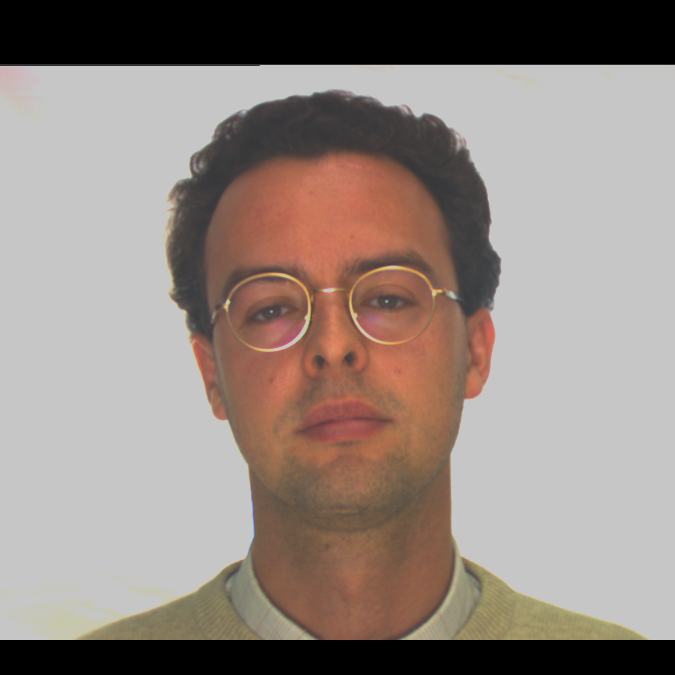
\includegraphics[width=0.23\linewidth]{images/washed_out/AR_m-007-1_C40.png}}
\hfill
\subfigure{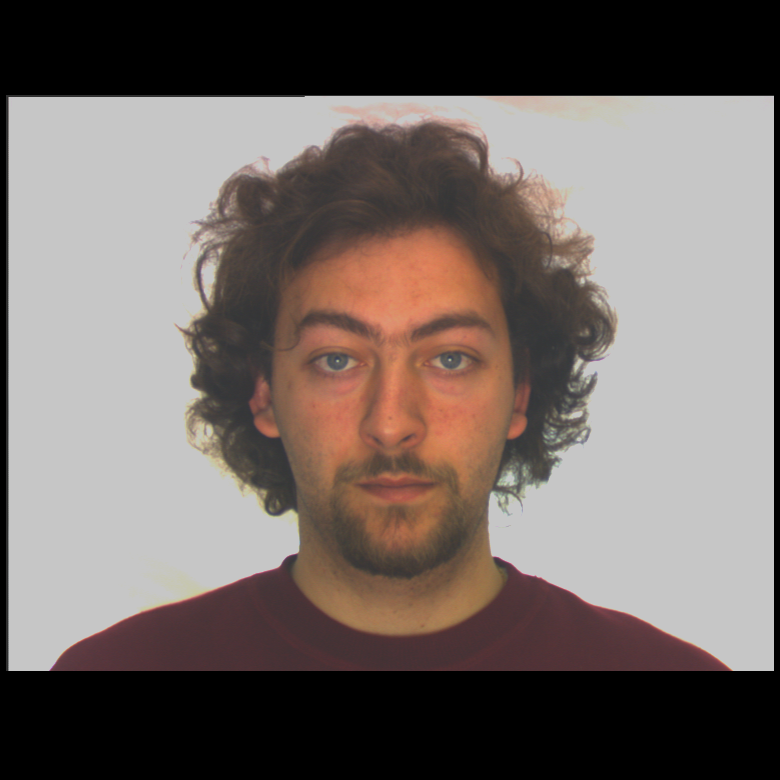
\includegraphics[width=0.23\linewidth]{images/washed_out/AR_m-048-1_C40.png}}
\hfill
\subfigure{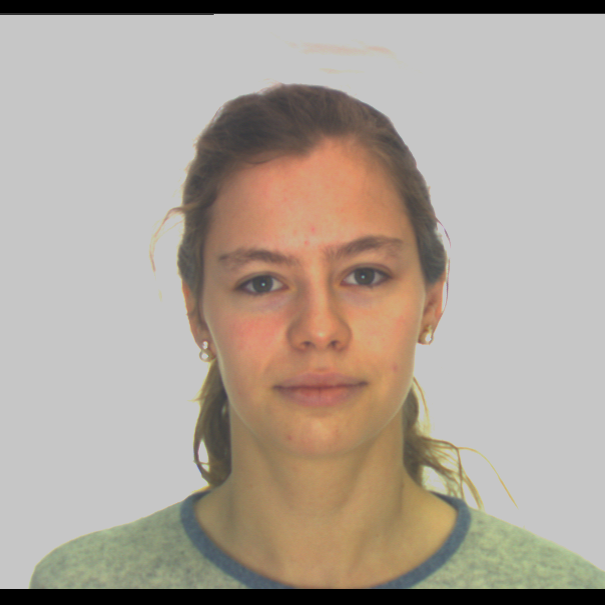
\includegraphics[width=0.23\linewidth]{images/washed_out/AR_w-018-1_C40.png}}
\hfill
\subfigure{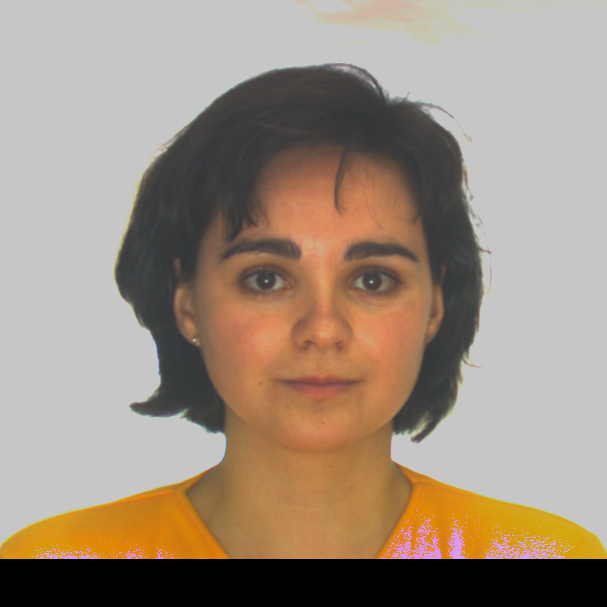
\includegraphics[width=0.23\linewidth]{images/washed_out/AR_w-054-1_C40.png}}
\caption{Example of preprocessed non-compliant images from the \washedout requirement. Source: own elaboration.}
\label{fig:washedout}
\end{figure}

\begin{figure}[t]
\centering
\subfigure[original image]{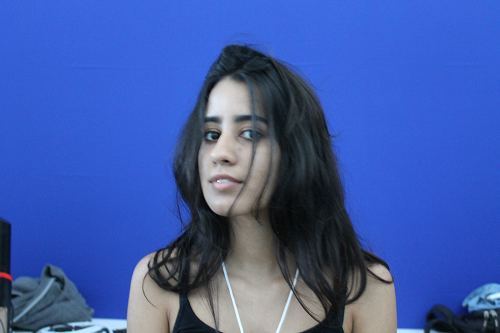
\includegraphics[height=1.5in]{images/varied_background/visio_icao_expotec_56.png}}
\hspace{0.5in}
\subfigure[preprocessed image]{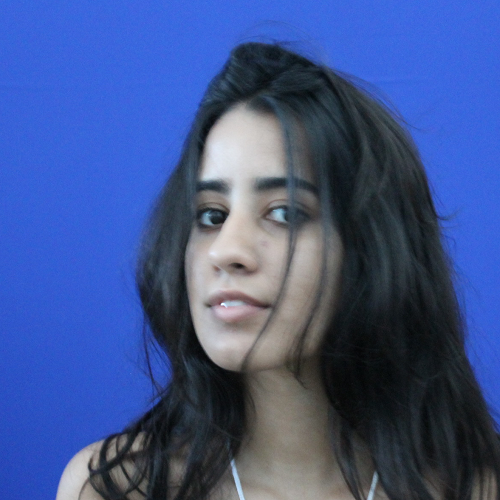
\includegraphics[height=1.5in]{images/varied_background/visio_icao_expotec_56_preprocessed.png}}
\caption{Example of a non-compliant image from the \variedbackground requirement before and after the preprocessing step. Source: own elaboration.}
\label{fig:variedbgd}
\end{figure}

\begin{figure}[t]
\centering
\subfigure[before resize (1715x1715)]{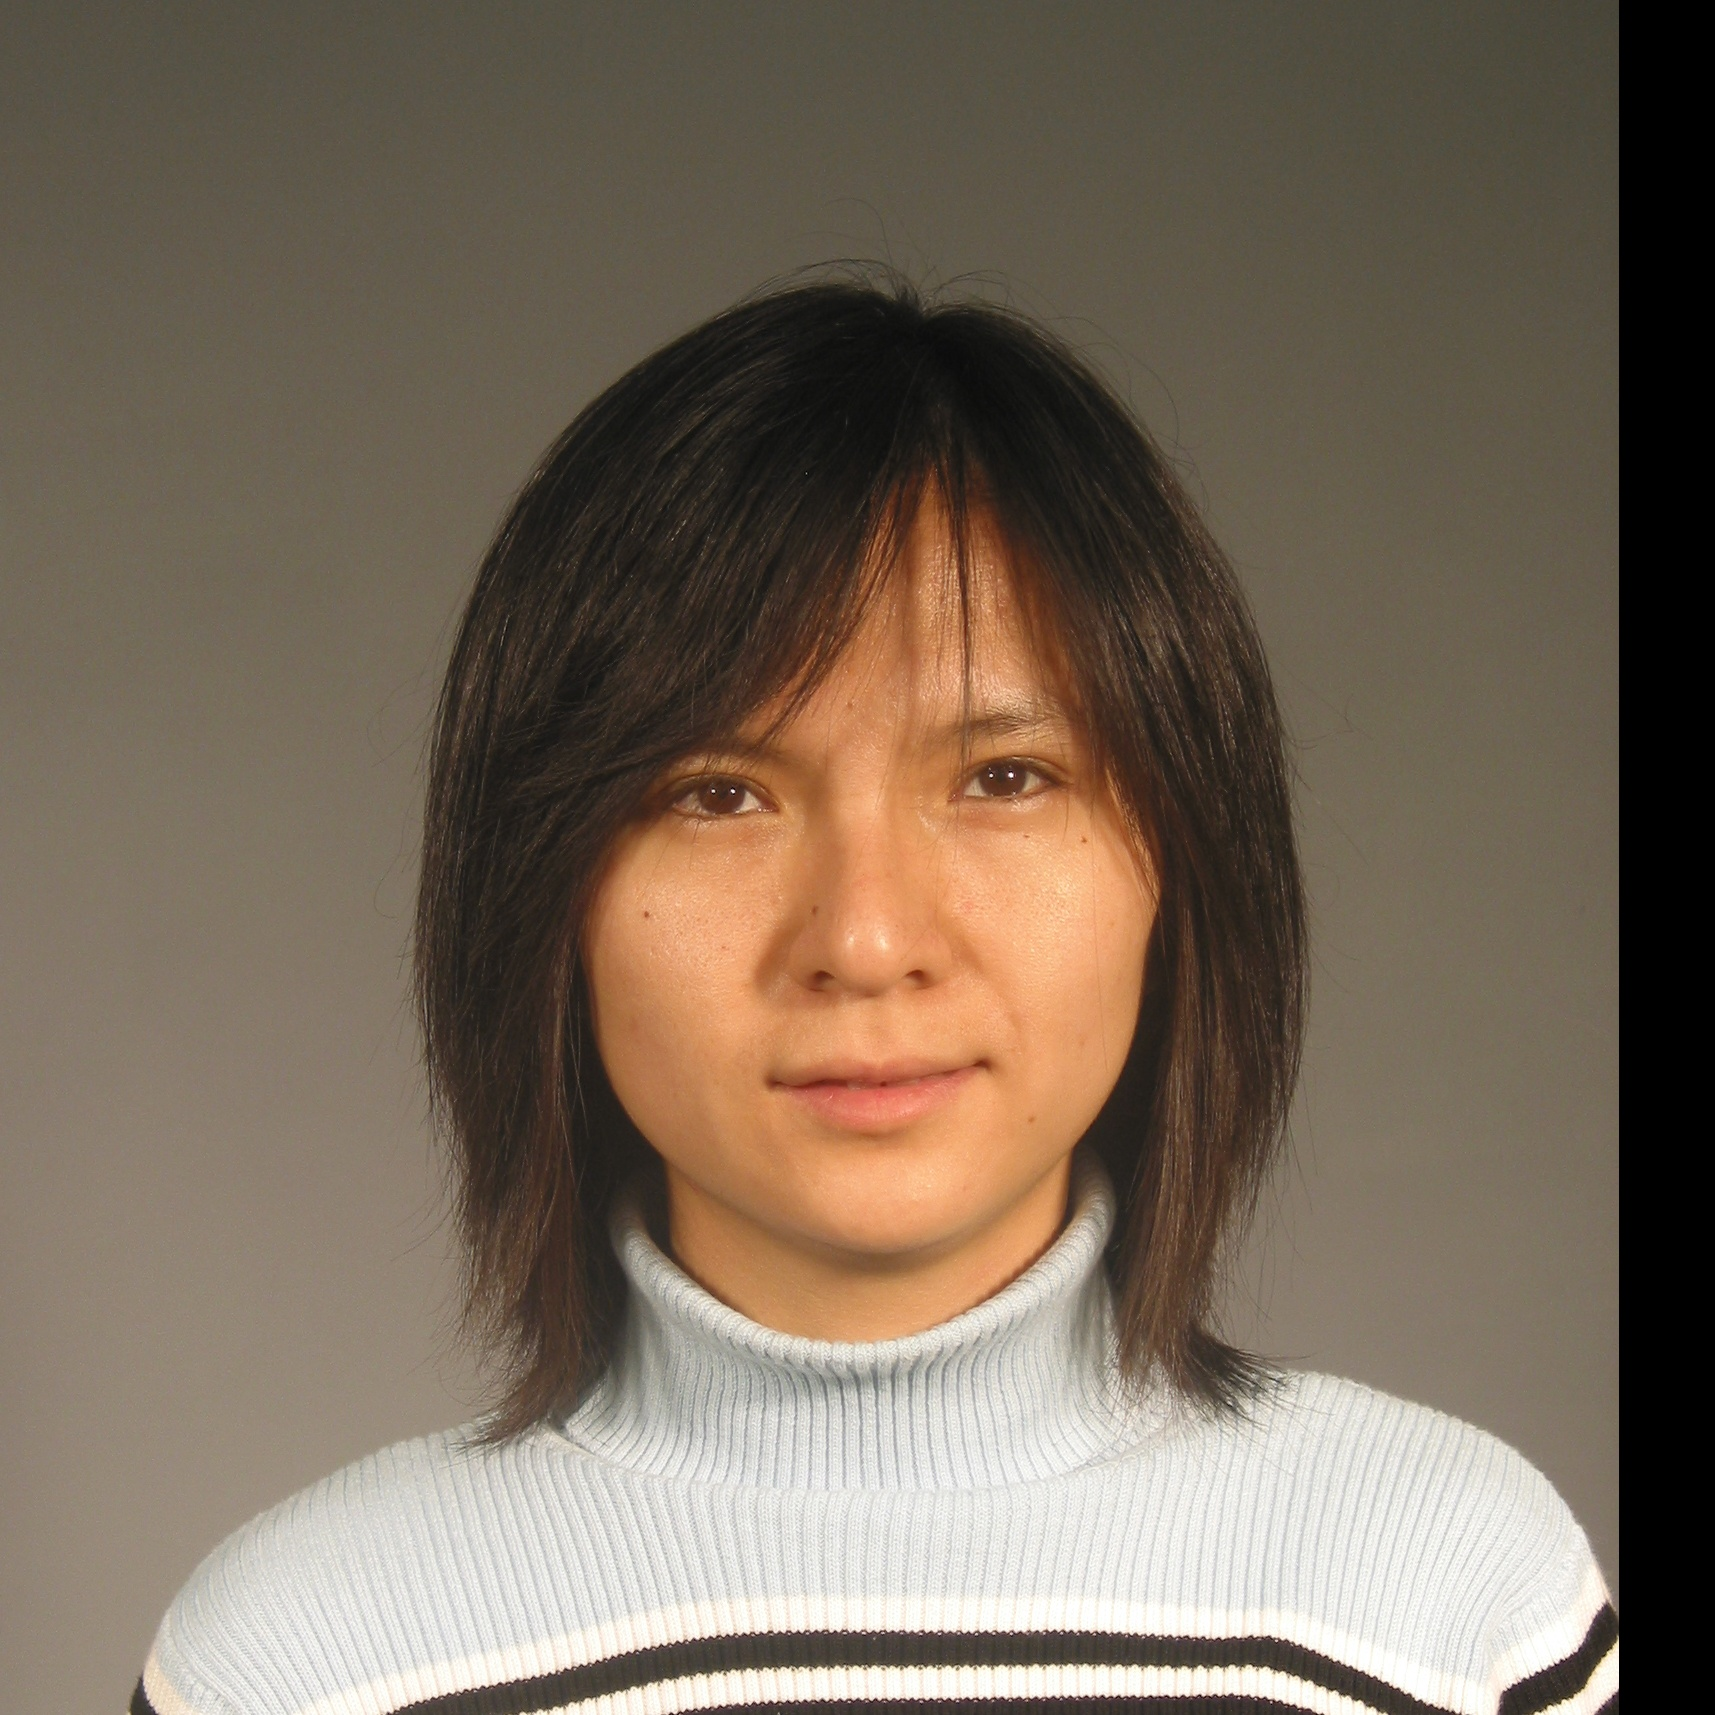
\includegraphics[height=2in]{images/hair_across_eyes/Fall2003_04853d17_preprocessed.jpg}}
\hspace{0.5in}
\subfigure[after resize (160x160)]{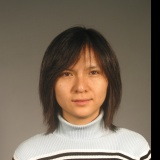
\includegraphics[height=2in]{images/hair_across_eyes/Fall2003_04853d17_resized.jpg}}
\caption{Example of a non-compliant image from the \hairacrosseyes requirement before and after the resizing operation performed by the preprocessing step. Source: own elaboration.}
\label{fig:hairacrosseyes}
\end{figure}

The \autoref{fig:eer_unbalancing} shows the \acs{eer} in both FICV datasets (as in \autoref{tab:icaonet-ficv}), but ordering the requirements by the proportion of non-compliant images in the ad-hoc dataset. Through the analysis of this graph, we can make some conclusions. First, as pointed before, the performance on both datasets is similar to each other. It reinforces the premise of FICV that the \ficvtest is a representative set of the \ficvofficial dataset (see section \ref{sec:fvcongoing}). Secondly, there is a moderate correlation between the EER and the degree of unbalancing in our dataset. According to Pearson's correlation, these coefficients are -0.47 and -0.45 for the \ficvtest and \ficvofficial datasets, respectively. In other words, if the proportion of non-compliant images increases, the \acs{eer} tends to decrease. However, it is important to notice that the fifth most unbalanced requirement (\veiloverface), with only 364 non-compliant images (or 6.31\%), is the one that achieved 0.0\% of \acs{eer} in both datasets. Also, these correlations become very weak and positives ($< +0.1$) when computed starting from the seventh most unbalanced requirement (\toodarklight, with 456 non-compliant images or 7.91\%).

\begin{figure}[ht]
\centering
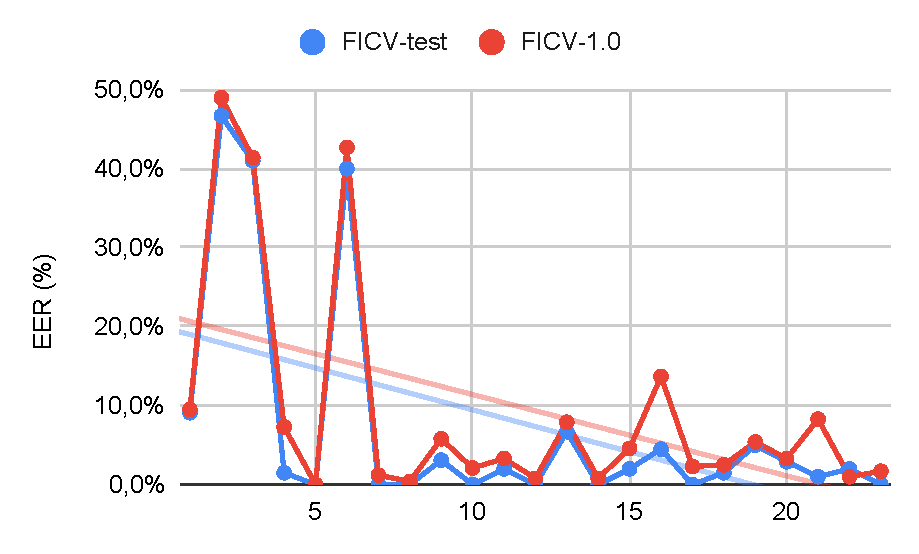
\includegraphics[width=0.8\linewidth]{images/graphs/eer_unbalancing.pdf}
\caption{EER by the proportion of non-compliant images for each requirement in ascending order. Source: own elaboration.}
\label{fig:eer_unbalancing}
\end{figure}

Regarding the eye location accuracy, the results in \acs{ficv} can be seen in \autoref{tab:eyes_ficv}. In both datasets of the competition, the results were close to the observed locally during training ($d_{eye} \in [0;0.1[ = 46.18\%$, see Section \ref{sec:eye_location_acc}). Even though $d_{eye} \in [0;0.1[$ is not as high as expected, we can notice that $d_{eye} \leq 0.2$ of \methodname is higher than $90\%$ in both official datasets. Hence, if we can improve the landmark detection of our method, acceptable levels of eye locations accuracy can be accomplished. Despite of it, significant results of tokenizable were achieved already.

% Please add the following required packages to your document preamble:
% \usepackage{booktabs}
% \usepackage{graphicx}
\begin{table}[tb]
\centering
\caption{Results of eye localization accuracy for \methodname in the official datasets of FICV competition.}
\label{tab:eyes_ficv}
\resizebox{\textwidth}{!}{%
\begin{tabular}{@{}rrrrrrr@{}}
\toprule
\textbf{} &
  \textbf{$d_{eye} \in [0;0.1[$} &
  \textbf{$d_{eye} \in [0.1;0.2[$} &
  \textbf{$d_{eye} \in [0.2;0.3[$} &
  \textbf{$d_{eye} \geq 0.3$} &
  \textbf{Rejected} &
  \textbf{Tokenizable} \\ \midrule
\ficvtest &
  43.59\% &
  46.80\% &
  4.80\% &
  4.80\% &
  0.00\% &
  88.97\% \\
\ficvofficial &
  42.68\% &
  48.24\% &
  5.46\% &
  3.62\% &
  0.00\% &
  89.19\% \\ \bottomrule
\end{tabular}%
}
\end{table}

\subsubsection{Analysis of the Worst Requirements}

% Trazer análise dos piores resultados para cá (linha 35: Three requirements had an \acs{eer} greater than 40\%) 
% e mencionar as tentativas de melhoria
% colocar um asterisco no resultado de Pixelation da tabela 6 com uma nota de rodapé, indicando que aquele resultado foi melhorado e citando esse seção

\subsection{Comparison Against Other Methods}

We start by comparing the results of \methodname with well-known architectures fine-tuned for \icao requirements. Because of the \acs{ficv} constraint for submission files (up to 50MB, see Section \ref{sec:fvcongoing}), only three architectures could be evaluated in the competition: MobileNet v1/v2 and NasNetMobile. As can be seen in \autoref{tab:comp_finetune}, \methodname outperforms the other architectures in almost all requirements (18 out of 23). There is a draw for \veiloverface, in which MobileNet v1/v2 and our method achieved 0\% of EER. Also, MobileNet v1 was able to achieve the best results in 3 other requirements (\pixelation, \hatcap, and \otherfacesortoys), while NasNet had the worst results within all methods compared. In addition, \methodname obtained the lowest results in terms of mean/median \acs{eer}, running time, and memory consumption. Finally, by these results, we can conclude the \acl{mtl} approach employed by the method proposed can perform better in practice than some networks fine-tuned for \icao.

A detailed analysis of the results shown in \autoref{tab:comp_finetune} can expose some interesting patterns. First, we can cite the eyes-related requirements. For \lookingaway, \eyesclosed, \redeyes, \darktintedlenses, \flashlenses, \framestooheavy, and \framecoveringeyes, our method achieved considerable improvements in terms of \acs{eer} (more than 50\% lower). In fact, the only requirement related to eyes that our method accomplished similar results with the other architectures was \hairacrosseyes. As mentioned before (see Section \ref{sec:ficv_results}), this results was probably influenced by our preprocessing step. We can also observe noticeable improvements for light-related requirements as \toodarklight, \shadowsbehindhead and \shadowsacrossface. Finally, when considering the highest unbalanced requirements, the proposed method also accomplished high \acs{eer} values for \inkmarked and \otherfacesortoys, but substantially lower values for \washedout and \framestooheavy.

% Please add the following required packages to your document preamble:
% \usepackage{graphicx}
\begin{table}[tb]
\centering
\caption{Comparison of the \methodname against fine-tuned versions of well-known architectures in \ficvofficial dataset.}
\label{tab:comp_finetune}
\resizebox{\textwidth}{!}{%
\begin{tabular}{clrrrr}
\hline
\textbf{Req. \#} &
  \textbf{Requirement description} &
  \multicolumn{1}{c}{\textbf{\begin{tabular}[c]{@{}c@{}}MobileNet\\ v1\end{tabular}}} &
  \multicolumn{1}{c}{\textbf{\begin{tabular}[c]{@{}c@{}}MobileNet\\ v2\end{tabular}}} &
  \multicolumn{1}{c}{\textbf{NasNet}} &
  \multicolumn{1}{c}{\textbf{\methodname}} \\ \hline
\textbf{08} & Blurred                           & 2.1           & \textbf{1.9} & 4.8   & 2.1           \\
\textbf{09} & Looking away                      & 17.3          & 26.3         & 23.1  & \textbf{5.4}  \\
\textbf{10} & Ink marked/creased                & 50            & 49.3         & 51.0  & \textbf{49.0} \\
\textbf{11} & Unnatural skin tone               & 18.5          & 19.0         & 24.0  & \textbf{1.7}  \\
\textbf{12} & Too dark/light                    & 7.7           & 7.1          & 6.7   & \textbf{1.2}  \\
\textbf{13} & Washed out                        & 15.6          & 12.3         & 23.7  & \textbf{7.3}  \\
\textbf{14} & Pixelation                        & \textbf{24.2} & 30.7         & 27.3  & 29.0          \\
\textbf{15} & Hair across eyes                  & 15.2          & 14.8         & 21.5  & \textbf{13.7} \\
\textbf{16} & Eyes closed                       & 9.2           & 14.8         & 24.2  & \textbf{0.8}  \\
\textbf{17} & Varied Background                 & 9.4           & 10.4         & 13.7  & \textbf{8.3}  \\
\textbf{18} & Roll/pitch/yaw                    & 10.6          & 9.6          & 24.5  & \textbf{4.6}  \\
\textbf{19} & Flash reflection on skin          & 8.3           & 6.7          & 12.9  & \textbf{1.0}  \\
\textbf{20} & Red eyes                          & 28.7          & 21.5         & 14.9  & \textbf{7.9}  \\
\textbf{21} & Shadows behind head               & 13.3          & 11.4         & 15.8  & \textbf{3.3}  \\
\textbf{22} & Shadows across face               & 12.1          & 12.1         & 12.7  & \textbf{3.3}  \\
\textbf{23} & Dark tinted lenses                & 1.0           & 1.5          & 1.2   & \textbf{0.4}  \\
\textbf{24} & Flash reflection on lenses        & 1.7           & 2.5          & 3.3   & \textbf{0.8}  \\
\textbf{25} & Frames too heavy                  & 50.0          & 45.3         & 35.1  & \textbf{9.5}  \\
\textbf{26} & Frame covering eyes               & 19.6          & 19.6         & 26.2  & \textbf{2.5}  \\
\textbf{27} & Hat/cap                           & \textbf{0.6}  & 1.9          & 1.0   & 5.8           \\
\textbf{28} & Veil over face                    & \textbf{0.0}  & \textbf{0.0} & 0.2   & \textbf{0.0}  \\
\textbf{29} & Mouth open                        & 11.7          & 11.7         & 17.7  & \textbf{2.3}  \\
\textbf{30} & Presence of other faces           & \textbf{36.7} & 45.5         & 48.4  & 41.4          \\ \hline
            & \multicolumn{1}{r}{mean (\%)}      & 15.8          & 16.4         & 18.9  & \textbf{8.8}  \\
            & \multicolumn{1}{r}{median (\%)}    & 12.1          & 12.1         & 17.7  & \textbf{3.3}  \\
            & \multicolumn{1}{r}{avg. time (s)} & 2.9           & 3.1          & 4.2   & \textbf{1.8}  \\
            & \multicolumn{1}{r}{max. time(s)}  & 3.4           & 4.2          & 5.2   & \textbf{3.3}  \\
            & \multicolumn{1}{r}{memory (MB)}   & 332.2         & 322.5        & 377.5 & \textbf{313} 
\end{tabular}%
}
\end{table}

Table \ref{tab:best-results} summarizes the best results by requirement among all the methods shown in Table \ref{tab:comp}. Also, it includes the results of \methodname for easy comparison. All methods were evaluated using the FICV competition benchmark tool and the official dataset (\ficvofficial). As can be seen, the proposed method has the best results in 9 out of 23 requirements of the \icao standard. Thus, the proposed method has the highest amount of best results in terms of requirements. We can also notice that \methodname has low rejection rates, with only four requirements rejecting at most 0.4\% of the evaluated images. Such rejections represent the false negatives from the face detector used to preprocess input images.

% Please add the following required packages to your document preamble:
% \usepackage[table,xcdraw]{xcolor}
% If you use beamer only pass "xcolor=table" option, i.e. \documentclass[xcolor=table]{beamer}
\begin{table}[!tb]
\centering
\caption{Comparison of the \methodname against the best results reported in the literature and by private SDK tools (see Table \ref{tab:comp}). All methods were evaluated by the benchmark tool of FICV using the \ficvofficial dataset.}
\label{tab:best-results}
\begin{tabular}{ccrrrr}
\hline
 & \multicolumn{3}{c}{\textbf{\begin{tabular}[c]{@{}c@{}}Best of Literature/\\ Commercial SDK\end{tabular}}} & \multicolumn{2}{c}{\textbf{ICAONet}} \\ \hline
\textbf{Req. \#} & Method & \multicolumn{1}{c}{EER} & \multicolumn{1}{c|}{{\color[HTML]{9B9B9B} Rej.}} & \multicolumn{1}{c}{EER} & \multicolumn{1}{c}{{\color[HTML]{9B9B9B} Rej.}} \\ \cline{2-6} 
\textbf{08} & BioPass Face & 1.60 & {\color[HTML]{9B9B9B} 3.30} & 2.10 & {\color[HTML]{9B9B9B} 0.60} \\
\textbf{09} & HMAX & 10.00 & {\color[HTML]{9B9B9B} 0.16} & \textbf{5.40} & {\color[HTML]{9B9B9B} 0.00} \\
\textbf{10} & BioLab & 3.40 & {\color[HTML]{9B9B9B} 1.20} & 49.00 & {\color[HTML]{9B9B9B} 0.00} \\
\textbf{11} & BioPass Face & 1.90 & {\color[HTML]{9B9B9B} 0.00} & \textbf{1.70} & {\color[HTML]{9B9B9B} 0.00} \\
\textbf{12} & id3 & 2.90 & {\color[HTML]{9B9B9B} 0.00} & \textbf{1.20} & {\color[HTML]{9B9B9B} 0.00} \\
\textbf{13} & BioPass Face & 0.00 & {\color[HTML]{9B9B9B} 0.00} & 7.30 & {\color[HTML]{9B9B9B} 0.00} \\
\textbf{14} & SDK 2 & 0.00 & {\color[HTML]{9B9B9B} 0.00} & 29.00 & {\color[HTML]{9B9B9B} 0.00} \\
\textbf{15} & Parente et al. & {\color[HTML]{333333} 11.90} & {\color[HTML]{9B9B9B} 3.40} & 13.70 & {\color[HTML]{9B9B9B} 0.40} \\
\textbf{16} & id3 & 0.20 & {\color[HTML]{9B9B9B} 1.00} & 0.80 & {\color[HTML]{9B9B9B} 0.00} \\
\textbf{17} & BioTest & 3.70 & {\color[HTML]{9B9B9B} 7.90} & 8.40 & {\color[HTML]{9B9B9B} 1.30} \\
\textbf{18} & id3 & 9.10 & {\color[HTML]{9B9B9B} 6.90} & \textbf{4.60} & {\color[HTML]{9B9B9B} 0.20} \\
\textbf{19} & BioLab & 0.60 & {\color[HTML]{9B9B9B} 0.00} & 1.00 & {\color[HTML]{9B9B9B} 0.00} \\
\textbf{20} & id3 & 1.00 & {\color[HTML]{9B9B9B} 2.00} & 8.20 & {\color[HTML]{9B9B9B} 1.50} \\
\textbf{21} & BioLab & 2.30 & {\color[HTML]{9B9B9B} 0.20} & 3.30 & {\color[HTML]{9B9B9B} 0.00} \\
\textbf{22} & Andrezza et al. & 7.70 & {\color[HTML]{9B9B9B} 2.50} & \textbf{3.30} & {\color[HTML]{9B9B9B} 0.20} \\
\textbf{23} & BioPass Face & 1.80 & {\color[HTML]{9B9B9B} 1.20} & \textbf{0.40} & {\color[HTML]{9B9B9B} 0.00} \\
\textbf{24} & BioLab & 2.10 & {\color[HTML]{9B9B9B} 0.00} & \textbf{0.80} & {\color[HTML]{9B9B9B} 0.00} \\
\textbf{25} & HMAX & 0.00 & {\color[HTML]{9B9B9B} 0.00} & 9.50 & {\color[HTML]{9B9B9B} 0.00} \\
\textbf{26} & HMAX & 0.00 & {\color[HTML]{9B9B9B} 0.10} & 2.30 & {\color[HTML]{9B9B9B} 0.60} \\
\textbf{27} & id3 & 6.80 & {\color[HTML]{9B9B9B} 0.80} & \textbf{5.70} & {\color[HTML]{9B9B9B} 0.20} \\
\textbf{28} & Parente et al. & 1.20 & {\color[HTML]{9B9B9B} 0.50} & \textbf{0.00} & {\color[HTML]{9B9B9B} 0.00} \\
\textbf{29} & id3 & 0.60 & {\color[HTML]{9B9B9B} 0.40} & 2.30 & {\color[HTML]{9B9B9B} 0.00} \\
\textbf{30} & BioPass Face & 1.20 & {\color[HTML]{9B9B9B} 2.70} & 41.40 & {\color[HTML]{9B9B9B} 0.00} \\ \hline
\multicolumn{4}{r}{\textbf{mean (\%)}} & 8.80 & 0.22 \\
\multicolumn{4}{r}{\textbf{median (\%)}} & 3.30 & 0.00 \\
\multicolumn{4}{r}{\textbf{avg. time (s)}} & \multicolumn{2}{c}{2.7} \\
\multicolumn{4}{r}{\textbf{max. time (s)}} & \multicolumn{2}{c}{3.4} \\
\multicolumn{4}{r}{\textbf{memory (MB)}} & \multicolumn{2}{c}{306.1}
\end{tabular}
\end{table}

There are four methods with public results published in the \fvcongoing: BioPass Face \citep{fvcVsoft}, BioTest \citep{fvcBioTest}, id3 \citep{fvcICAOCompliance}, and ICAOSDK \citep{fvcSeamfix}. In comparison to them, we have the best results in 11 out of all 23 requirements. Therefore, the \methodname is also the method with the highest amount of best results in terms of requirements in the FICV competition. Additionally, the proposed method has the second-best Median EER (3.3\%).

In terms of performance, the \methodname takes on average 1.8 seconds per image according to the official benchmark results on the FICV competition of the \fvcongoing website. In comparison with methods that evaluate all requirements, the proposed method is the fastest. However, according to our benchmarks, almost 90\% of the \methodname running time is dominated by the face detector (1.6s on average), which is a preprocessing step. On the other hand, the architecture of the proposed network takes only 0.15s of this total time. Furthermore, since the FICV competition runs the benchmarks in CPU-only computers, our network could be even faster by using a GPU. In the future, we intend to change our face detector to a faster alternative so that our total time in CPU will be reduced even more.

To improve these results, two distinct approaches can be followed. First, our dataset quality can be improved by increasing (i) the number of images and (ii) the variability of patterns of some requirements (like hat/cap). Thereby, the network can learn more effective descriptors and decrease our EER in these requirements. Secondly, we may change the network or try other loss functions. For instance, we can test loss functions designed for multi-label classification problems, like the Contrastive Loss \citep{khosla2020supervised}.

With respect to eye location accuracy, \autoref{tab:comp_eyes} compares the \methodname with the other methods published in the \acs{ficv} competition. Despite \methodname has the worst performance for $d_{eye} \in [0;0.1[$ ($42.68\%$), as discussed before, our $d_{eye} \leq 0.2$ is greater than 90\%. Thus, if we improve our landmark prediction, we can achieve performance results comparable to \biopass and id3 methods. Moreover, it is important to highlight that \methodname is the only method that does not reject images. Finally, the landmarks detected by our method are already able to allow the tokenization of almost 90\% of the input images, being better than \biotest algorithm.

We believe the most effective way to improve our landmark predictions is by improving our dataset. First, the amount of samples must be increased to follow other landmark datasets with hundreds of thousands images. Furthermore, the variation of landmarks is an important factor as well. It includes, for example, more face positions with a higher range of head rotations in all axis (which can not be achieved by classic image augmentation techniques). Lastly, we could also try other custom loss functions specially designed for landmark localization.

% Please add the following required packages to your document preamble:
% \usepackage{booktabs}
% \usepackage{graphicx}
\begin{table}[tb]
\centering
\caption{Results of eye localization accuracy for the methods with published results in the FICV competition.}
\label{tab:comp_eyes}
\resizebox{\textwidth}{!}{%
\begin{tabular}{@{}rrrrrrr@{}}
\toprule
\textbf{} &
  \textbf{$d_{eye} \in [0;0.1[$} &
  \textbf{$d_{eye} \in [0.1;0.2[$} &
  \textbf{$d_{eye} \in [0.2;0.3[$} &
  \textbf{$d_{eye} \geq 0.3$} &
  \textbf{Rejected} &
  \textbf{Tokenizable} \\ \midrule
\biopass    & 94.46\% &  2.00\% & 1.49\% & 0.65\% & 1.41\%  & 92.86\% \\
id3         & 95.46\% &  2.11\% & 0.73\% & 0.38\% & 1.32\%  & 95.03\% \\
\biotest    & 77.08\% &  5.08\% & 0.89\% & 2.73\% & 14.22\% & 78.22\% \\
\methodname & 42.68\% & 48.24\% & 5.38\% & 3.41\% &  0.30\% & 89.05\% \\ \bottomrule
\end{tabular}%
}
\end{table}

\subsection{Network Visualization} \label{sec:netviz}

In addition to the performance results already presented, we decided to apply different techniques to understand the network outputs. First, we analyzed the embeddings learned by the network using algorithms for dimensionality reduction. Secondly, we applied network visualization techniques to understand which image regions are the most relevant to each requirement. More details can be found in the following paragraphs.

A visualization of the embeddings learned by \methodname is shown in the 3D plots of Figure \ref{fig:embviz}. The embedding dimension was reduced to 3 dimensions and visualized via the PCA and t-SNE methods using TensorBoard\footnote{https://www.tensorflow.org/tensorboard}. Each point in the plot is represented by a face image from the dataset. Although the figure shows only three dimensions, it is possible to observe that some dimensions are related to particular ICAO requirements. For example, in the figure related to PCA, we can observe that images with \variedbackground, \unnaturalskintone, and \veiloverface are closer to each other in a certain degree. On the other hand, in t-SNE, we can notice that the clusters related to such requirements are more well defined, especially for \variedbackground and \veiloverface requirements. Moreover, in both figures, we can see the intersection between some regions. For instance, images with unnatural skin tone and veil over face tend to belong to both clusters. Such information is relevant to the multi-task classification branch of the \methodname architecture. 

\begin{figure}[ht]
\centering
\subfigure[PCA]{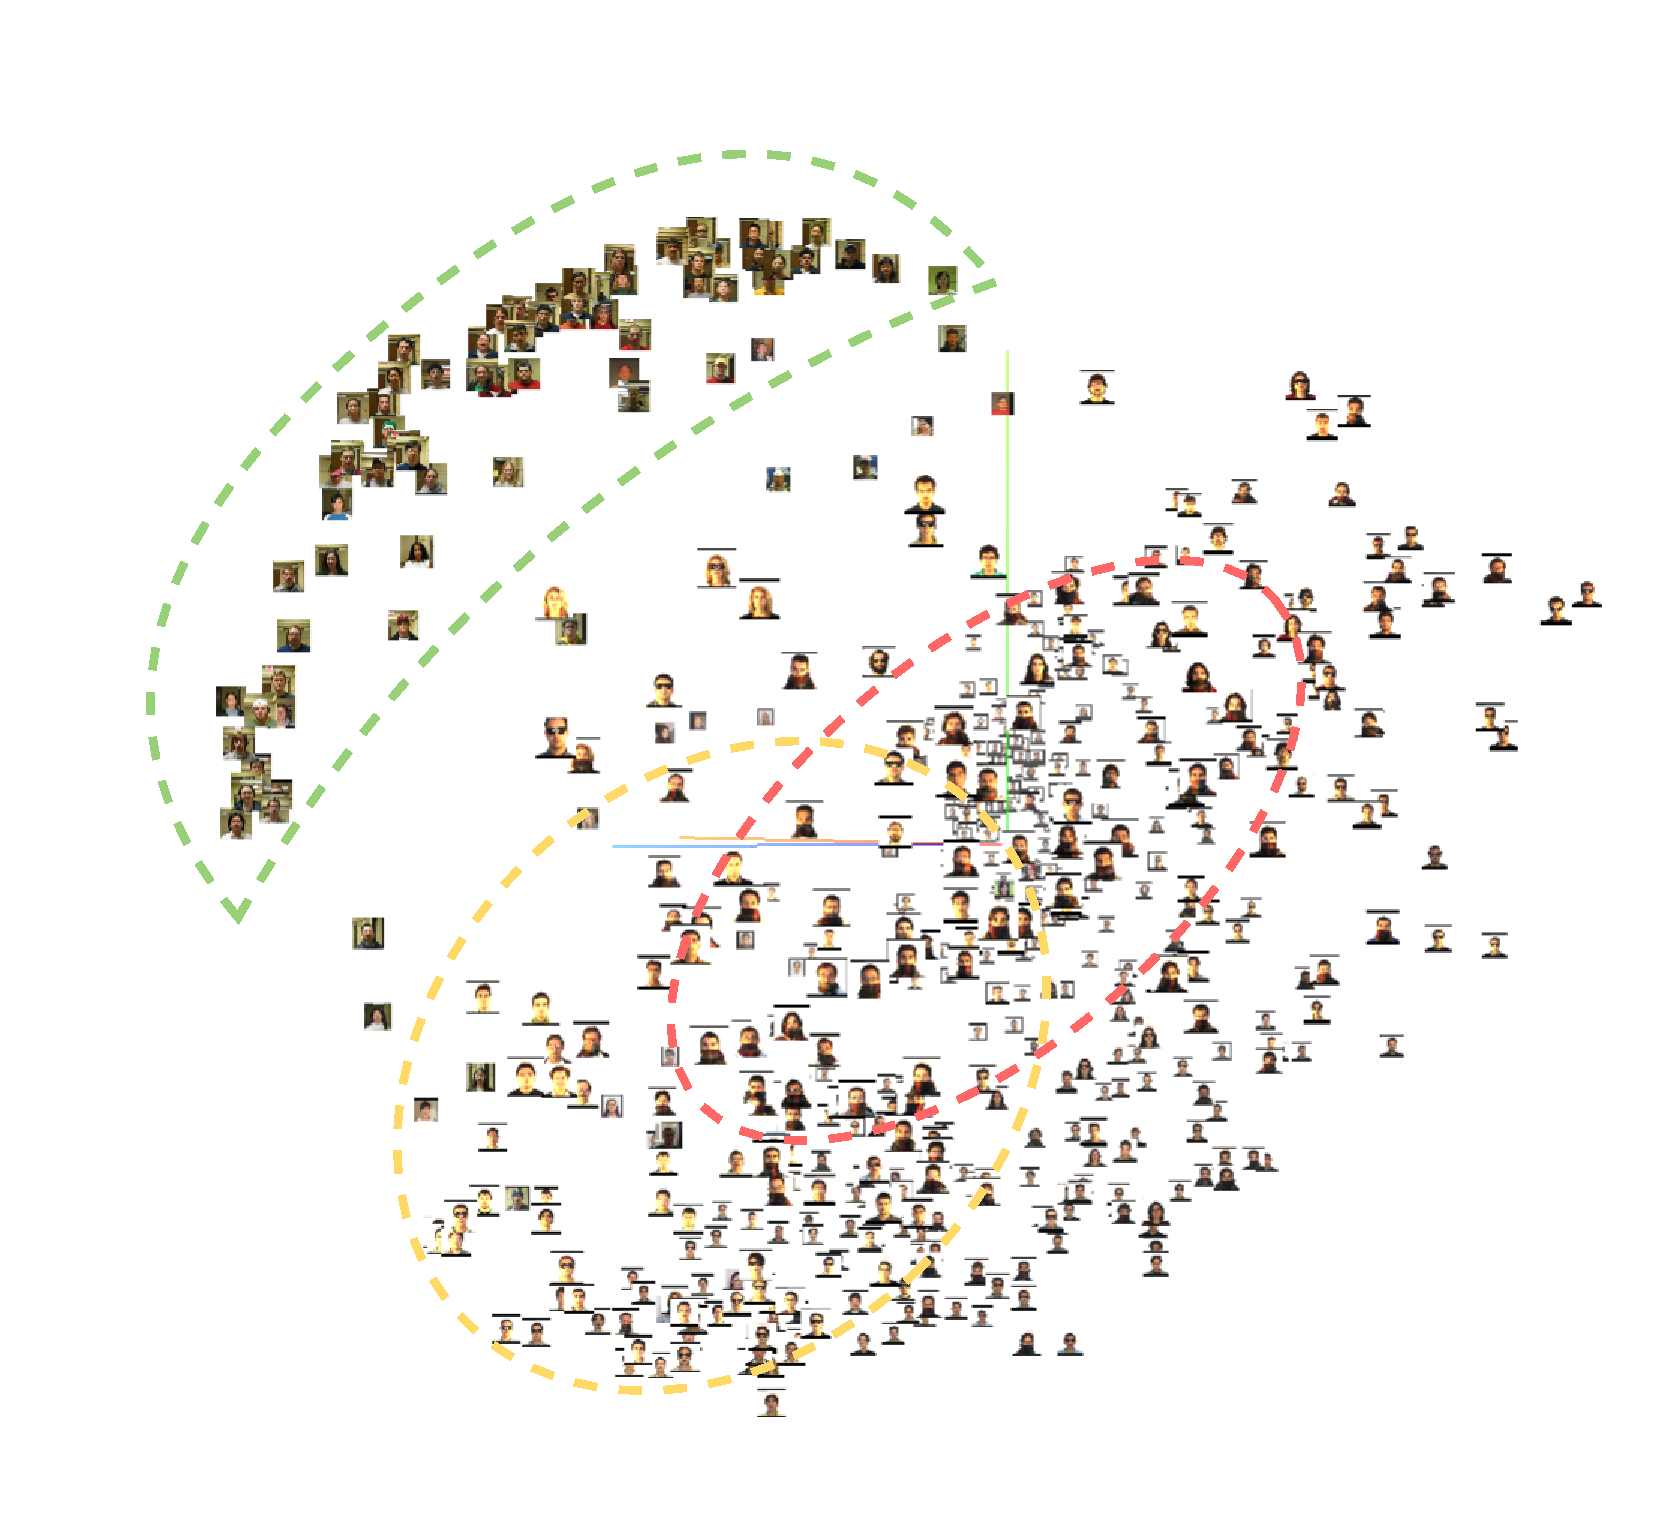
\includegraphics[width=0.75\linewidth]{images/pca.pdf}}
\subfigure[t-SNE]{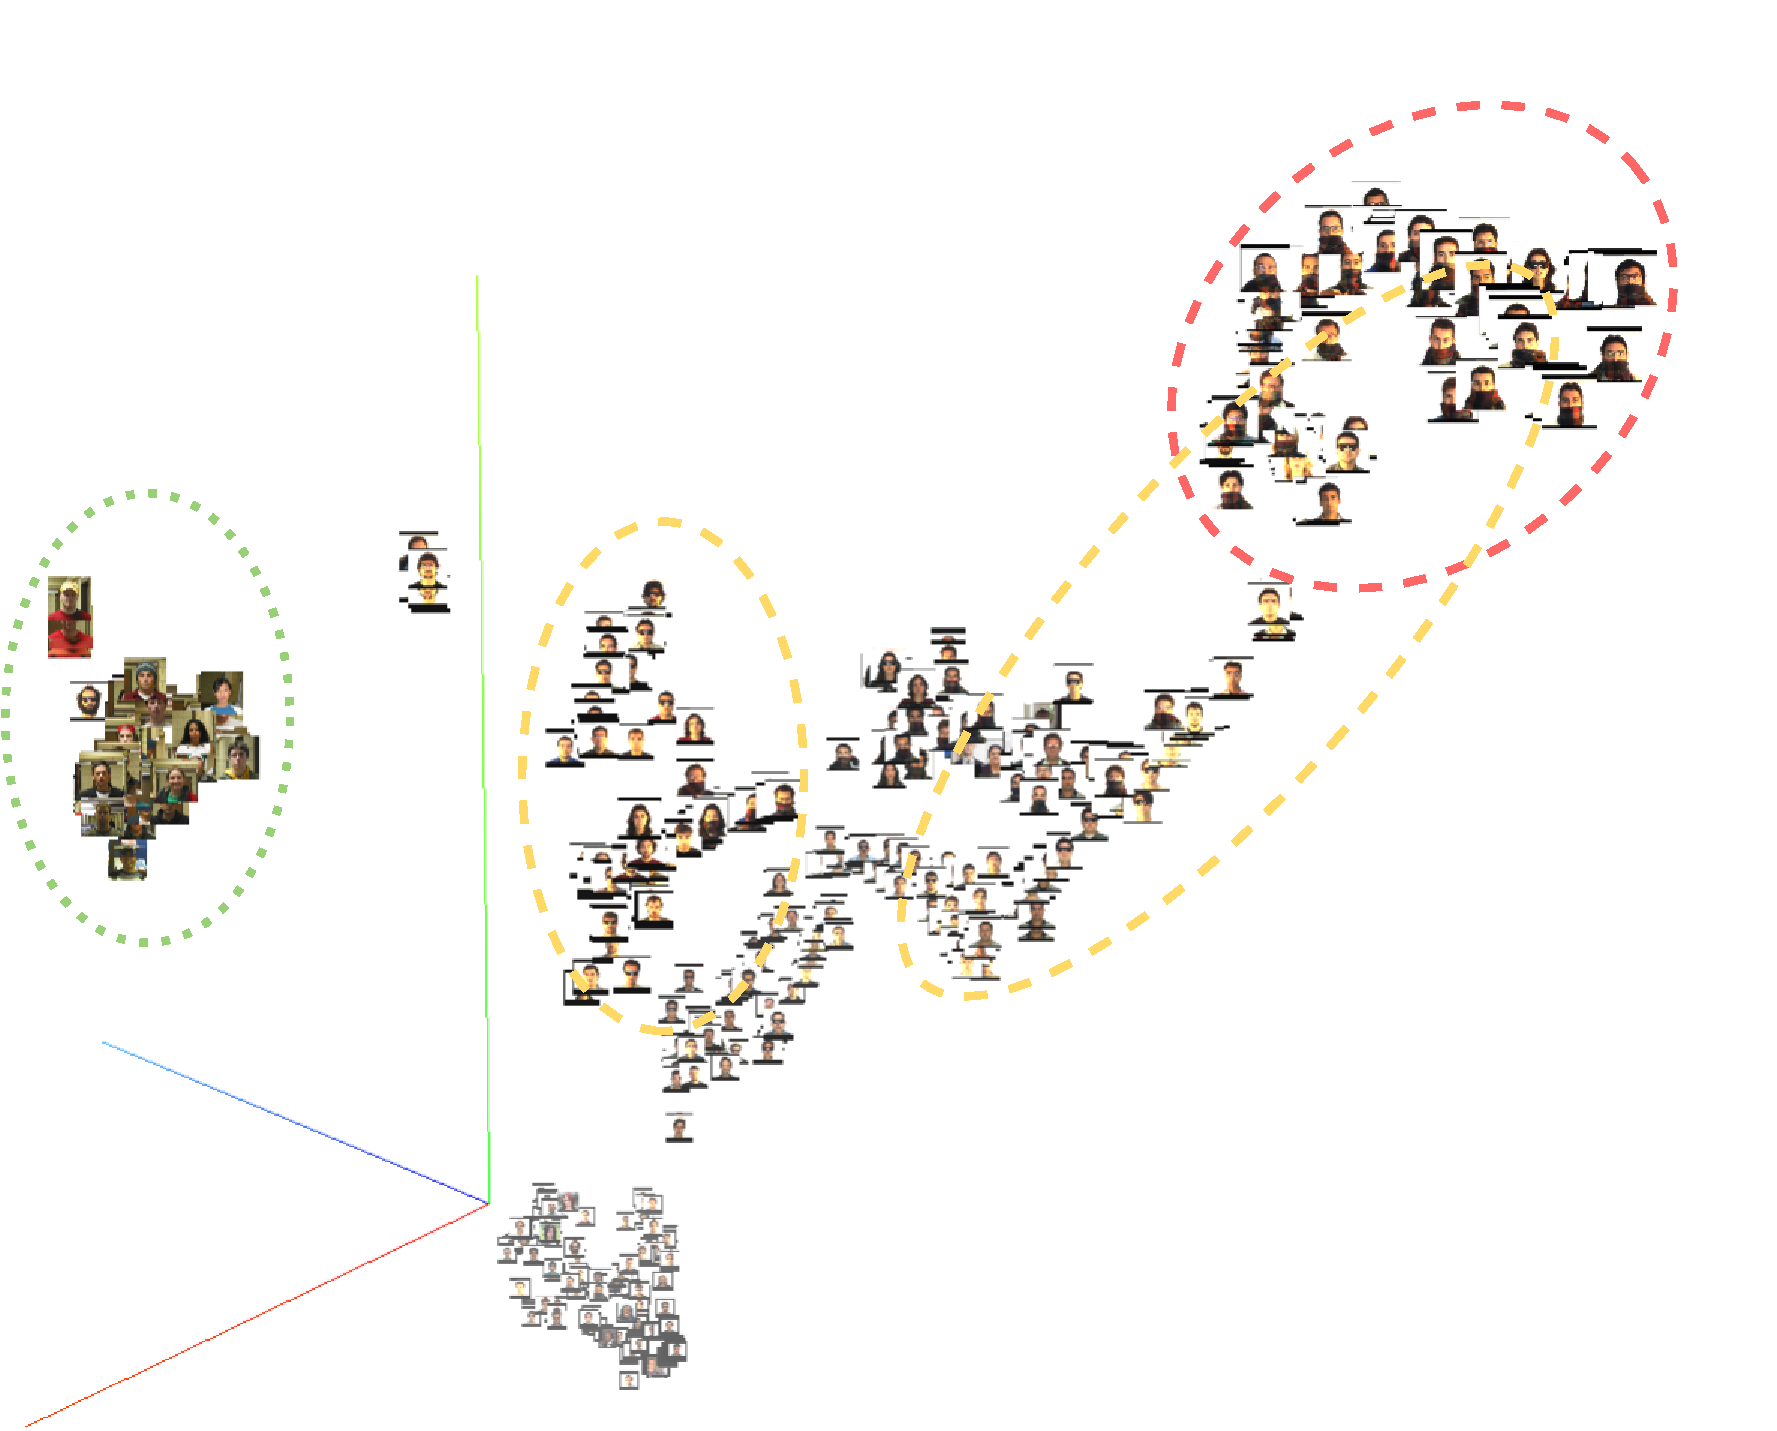
\includegraphics[width=0.75\linewidth]{images/tsne.pdf}}    
\caption{Visualization of the embeddings learned by \methodname. Original embeddings dimensions were reduced to 3D using (a) PCA and (b) t-SNE. In both visualizations, we highlight the regions of \variedbackground (green), \unnaturalskintone (yellow), and \veiloverface (red) requirements. Source: own elaboration.}
\label{fig:embviz}
\end{figure}

Figure \ref{fig:shap} contains a visual representation of input images with local region contributions associated with each pose and photograph requirements. The SHAP method was used to create that visualization. The figure provides evidence that the network learned useful representations for most of the requirements. In the fully compliant images (first three rows), the classification output is usually increased by the image regions related to that requirement. For example, in the eye-region dependent requirements (09, 15, 16, 20, 23, 24, and 26), the output is mainly influenced by regions closer to the eyes. Similar behaviors can be observed in requirements related to the mouth (28 and 29), skin (11, 19, 22), and the image aspect (08, 12, 13). 

However, we can notice the network was not able to learn relevant patterns in some requirements like \inkmarked, \pixelation, \framestooheavy, \hatcap, and \otherfacesortoys. For requirements 10, 25, and 30, we believe the low amount of non-compliant images was the most crucial factor in contributing to the worst results of the proposed architecture, found in Table \ref{tab:req-dist}. In the case of \pixelation, a possible cause for the high EER (42.7\%) could be the image resizing step applied in the input images. Finally, the random patterns in \hatcap may show that the variability of head props in our dataset must be insufficient to distinguish them from other patterns. 

\begin{landscape}
\begin{figure*}[ht]
\centering
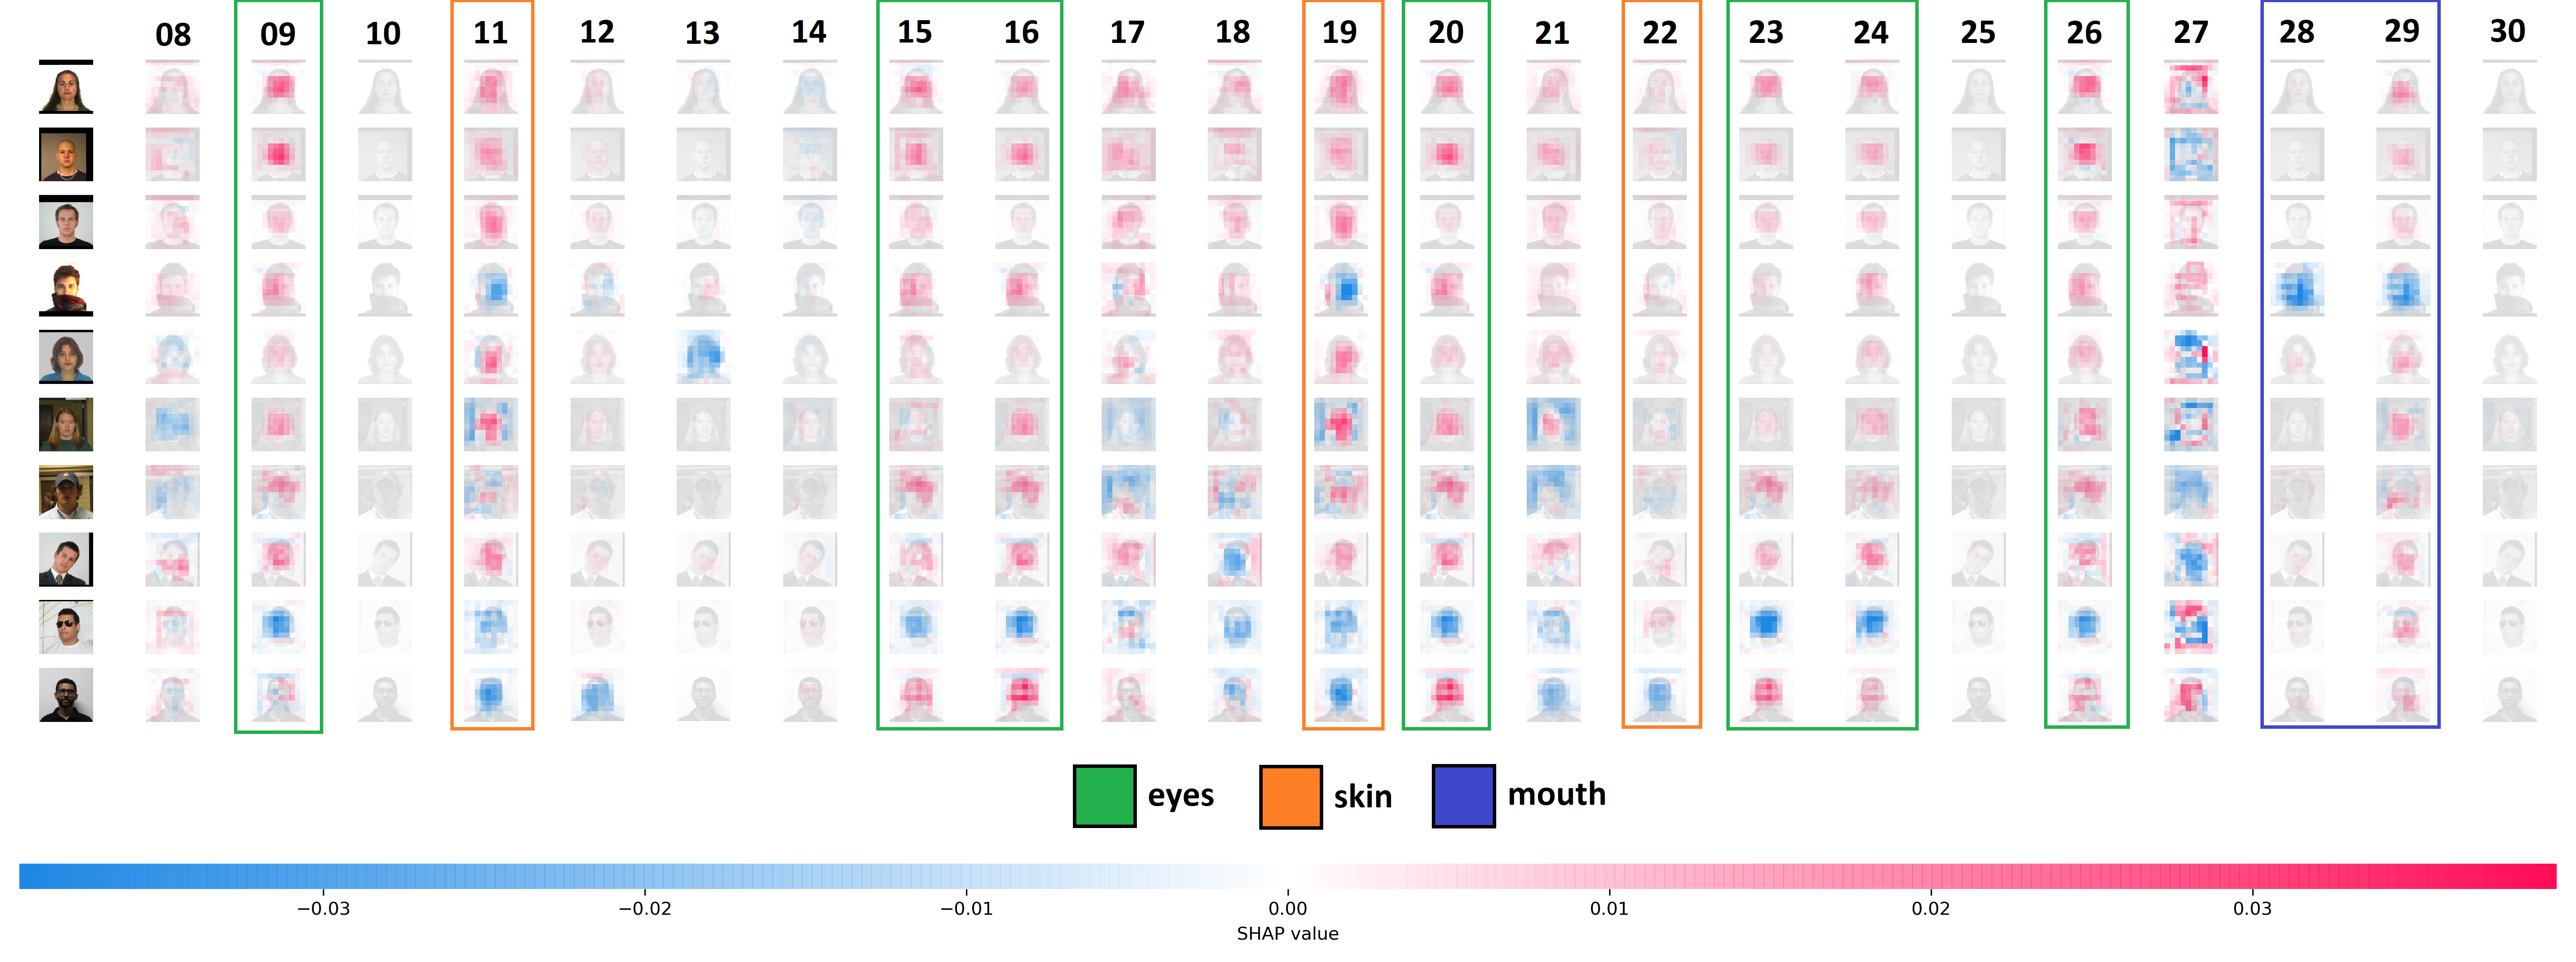
\includegraphics[width=\linewidth]{images/shap.png}
\caption{Visual explanation of \methodname's output using SHAP. The rows represent input images, and the columns denote the requirements from the \icao standard. The first three images are fully compliant, while the remaining images have at least one non-compliant requirement. According to the SHAP values, each pixel contributes negatively (blue), positively (red), or has a low contribution (white) to the network's output. Some requirements related to eyes, skin, and mouth are highlighted for convenience. Source: own elaboration.}
\label{fig:shap}
\end{figure*}
\end{landscape}
